\documentclass{standalone}
\usepackage{amsmath}
\usepackage{amssymb}
\usepackage{pgfplots}
\usepackage{tikz}

\begin{document}
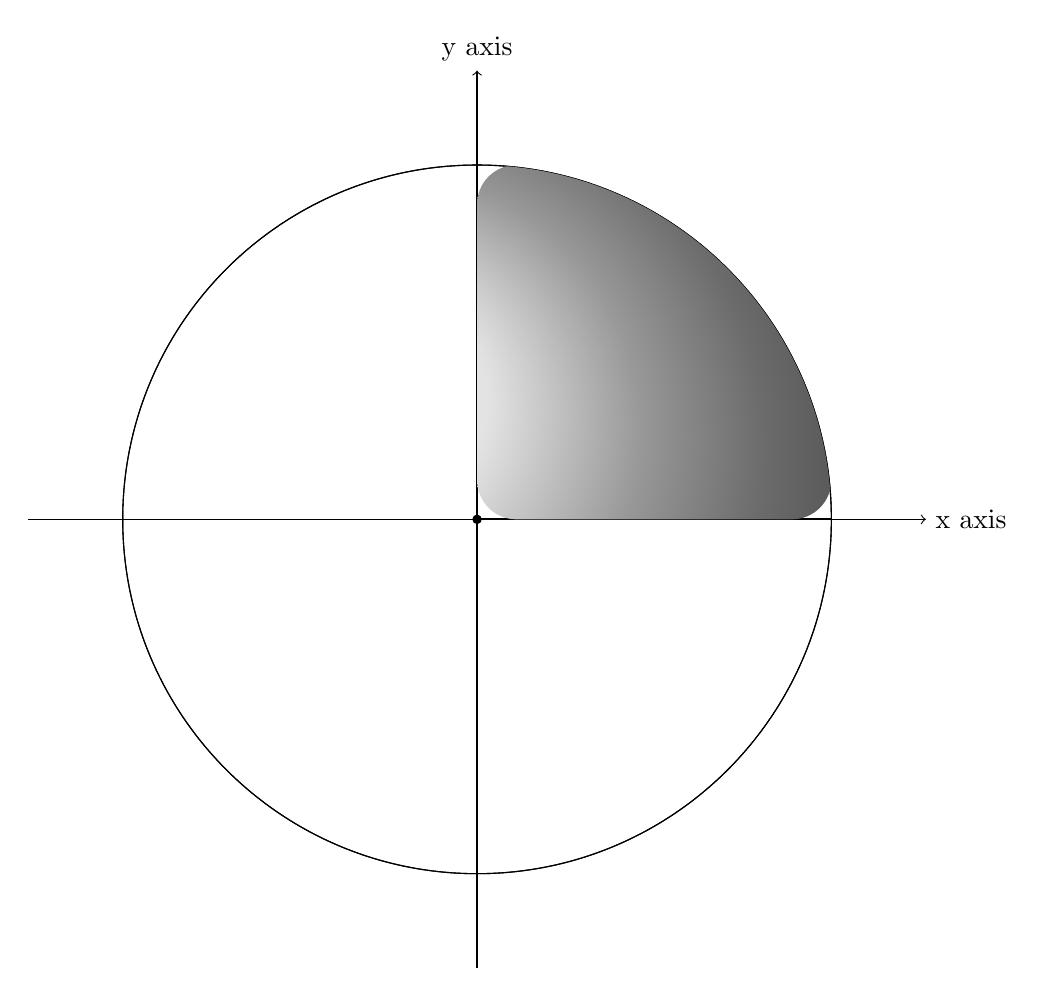
\begin{tikzpicture}[domain=-4:4,scale=1.5]
    \draw[->] (-3.8,0)--(3.8,0);
    \node[right] at (3.8,0){x axis};
    \draw[->] (0,-3.8)--(0,3.8);
    \node[above] at (0,3.8){y axis};
    \draw[thick] (0,0) -- (3,0);
    \draw[thick,dashed] (0,0) -- (3,0);
    \draw[thin] (0,0) circle [radius=3];
    \draw[thin] (0,0) circle [radius=3];
    \filldraw[black] (0,0) circle (1pt);
    \draw[dotted] (.7,.7) node{$\frac{M}{M+1}$};
    \filldraw[black] (.7,.7) circle (1pt);
    \begin{scope}[rounded corners=.5cm]
        \clip (0,0) rectangle (3,3);
        \shade[ball color=gray!30] (0,0) circle[radius=3];
    \end{scope}
\end{tikzpicture}
\end{document}